\documentclass[border=3pt]{standalone}
\usepackage{xcolor}
\usepackage{tikz}
\usetikzlibrary{arrows.meta,decorations.markings,positioning}

\definecolor{flowblue}{HTML}{2563EB}
\definecolor{floworange}{HTML}{EA580C}
\definecolor{flowink}{HTML}{1E293B}

\begin{document}
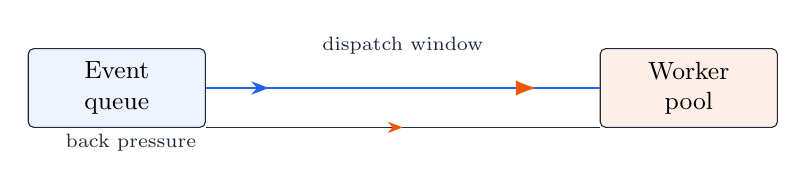
\begin{tikzpicture}[
  block/.style={draw=flowink,rounded corners=2pt,minimum width=2.25cm,
    minimum height=1cm,align=center,font=\small},
  note/.style={font=\scriptsize,text=flowink}
]
  \node[block,fill=flowblue!8] (queue) {Event\\queue};
  \node[block,fill=floworange!10,right=5cm of queue] (worker) {Worker\\pool};

  \draw[flowblue,line width=.75pt,postaction={decorate},
    decoration={markings,
      mark=at position 8mm with {\arrow{Stealth}},
      mark=at position -8mm with {\arrow[floworange,line width=1pt]{Latex}}}]
    (queue.east) -- node[note,above=3mm] {dispatch window} (worker.west);

  \draw[flowink,line width=.55pt,postaction={decorate},
    decoration={markings,
      mark=at position .5 with {\arrowreversed[floworange]{Stealth}}}]
    ([yshift=-5mm]worker.west) -- ([yshift=-5mm]queue.east);
  \node[note,below=7mm of queue.east,anchor=east] {back pressure};
\end{tikzpicture}
\end{document}
